\documentclass[12pt,a4paper]{article}

\usepackage[margin=2.5cm]{geometry}
\usepackage{amsmath,amssymb}
\usepackage[colorlinks=true,linkcolor=blue!55!black,citecolor=blue!55!black,urlcolor=blue!55!black]{hyperref}
\usepackage{booktabs}
\usepackage{graphicx}
\usepackage{xcolor}
\usepackage{fancyhdr}
\usepackage{siunitx}
\usepackage[utf8]{inputenc}
\usepackage[T1]{fontenc}
\usepackage{lmodern}
\usepackage[protrusion=true,expansion=true]{microtype}
\usepackage{titlesec}
\usepackage{caption}
\usepackage{placeins}

\frenchspacing
\widowpenalty=10000
\clubpenalty=10000
\setlength{\parindent}{0pt}
\setlength{\parskip}{0.8ex}

\titleformat{\section}{\normalfont\Large\bfseries}{\thesection}{1em}{}
\titleformat{\subsection}{\normalfont\large\bfseries}{\thesubsection}{1em}{}
\titlespacing*{\section}{0pt}{2.5ex plus 1ex minus .2ex}{1.3ex plus .2ex}
\titlespacing*{\subsection}{0pt}{2ex plus 1ex minus .2ex}{1ex plus .2ex}

\pagestyle{fancy}
\fancyhf{}
\setlength{\headheight}{14pt}
\renewcommand{\sectionmark}[1]{\markright{#1}}
\renewcommand{\subsectionmark}[1]{\markright{#1}}
\lhead{\small\nouppercase{\rightmark}}
\rhead{\small N-body gravitational simulation}
\cfoot{\thepage}
\renewcommand{\headrulewidth}{0.4pt}

\newcommand{\norm}[1]{\left\lVert#1\right\rVert}
\newcommand{\abs}[1]{\left|#1\right|}

\begin{document}

\hypersetup{pageanchor=false}
\begin{titlepage}
\thispagestyle{empty}
\centering
\vspace*{2cm}
{\scshape\Large The Hebrew University of Jerusalem\par}
\vspace{0.3cm}
{\scshape\large Department of Physics\par}
\vspace{2.5cm}
\rule{0.62\textwidth}{0.4pt}\par
\vspace{0.6cm}
{\Huge\bfseries N-body Gravitational Simulation\par}
\vspace{0.5cm}
{\LARGE Barnes--Hut tree with adaptive RK4\par}
\vspace{0.5cm}
\rule{0.62\textwidth}{0.4pt}\par
\vfill
{\large Eran Rehani\par}
\vspace{0.4cm}
{\large Course 77315: Computational Physics\par}
\vspace{0.4cm}
{\large 2026\par}
\vspace{2cm}
\end{titlepage}

\hypersetup{pageanchor=true}
\pagenumbering{roman}
\tableofcontents
\newpage
\pagenumbering{arabic}

\section{Problem and initial conditions}\label{sec:problem}

The simulation follows $N=5000$ equal-mass particles with total mass
$M=\num{1e11}\,M_\odot$ for \SI{20}{Gyr}. Initially, the particles are
distributed uniformly within a sphere of radius $R=\SI{50}{kpc}$. The sampler
uses $r=Ru_r^{1/3}$ and chooses an isotropic direction from
$\cos\vartheta=2u_\mu-1$ and $\varphi=2\pi u_\varphi$, with $u_r$, $u_\mu$ and
$u_\varphi$ drawn independently from $U(0,1)$.

Each velocity component follows a normal distribution with
$\sigma=V/\sqrt{3}$, so $V=\langle v^2\rangle^{1/2}$. The three runs use
$V=65$, $80$, and $\SI{95}{km/s}$. All three reuse the same positions and
standardized velocity draw; only the velocity scale changes. The initialization
routine subtracts the sampled mean velocity but leaves the positions unchanged,
keeping every particle inside the assigned sphere.

The assignment uses the softened force
\begin{equation}\label{eq:softforce}
 \mathbf{f}_{ij}=-\frac{Gm_im_j}{(r_{ij}+S)^2}
 \frac{\mathbf{r}_{ij}}{r_{ij}},
 \qquad \mathbf{r}_{ij}=\mathbf{r}_i-\mathbf{r}_j,
\end{equation}
with $S=\SI{1}{kpc}$. Its pair potential,
$U_{ij}=-Gm_im_j/(r_{ij}+S)$, defines the energy diagnostic. After each
accepted step, the solver removes particles with any coordinate outside the
$\pm\SI{666}{kpc}$ calculation box.

\section{Numerical method}\label{sec:method}

\subsection{Units}

The code uses kpc, $M_\odot$, and Gyr. In these units,
\begin{equation}
 G=\SI{4.4996e-6}{kpc^3.M_\odot^{-1}.Gyr^{-2}},
 \qquad \SI{1}{kpc/Gyr}=\SI{0.9777922}{km/s}.
\end{equation}
Each simulation particle has mass $m=M/N=\num{2e7}\,M_\odot$.

\subsection{Barnes-Hut tree}

The tree method follows Barnes and Hut \cite{barneshut}. At each force
evaluation, the tree builder places the particles in a cubic root cell and
splits every cell containing more than one particle into eight octants. Each
cell stores its particle count, mass, center of mass, and main diagonal
$L=\sqrt{3}\,l$. The brief defines $L$ as the diagonal, rather than the side
length $l$ used in the usual opening criterion.

For each target particle, the tree walk opens any cell that contains it and
evaluates a leaf by direct softened interaction, excluding self-interaction.
For an external cell at center-of-mass distance $D$, it recurses if
$D/L<\theta$ and replaces the cell by a point mass if $D/L\geq\theta$. The
solver uses the assigned $\theta=1$ and rebuilds the tree at every Runge-Kutta
stage.

Dividing Equation~\ref{eq:softforce} by the target mass gives one source's
acceleration,
\begin{equation}
 \mathbf{a}_{ij}=-\frac{Gm_j}{(r_{ij}+S)^2}
 \frac{\mathbf{r}_{ij}}{r_{ij}}.
\end{equation}
Small tests use a direct $O(N^2)$ calculation as the reference.
Figure~\ref{fig:tree} illustrates the same rules with a two-dimensional
quadtree. For this 60-particle example, the target requires 12 direct pairs and
14 cell terms instead of 59 direct pairs.

\begin{figure}[htbp]
 \centering
 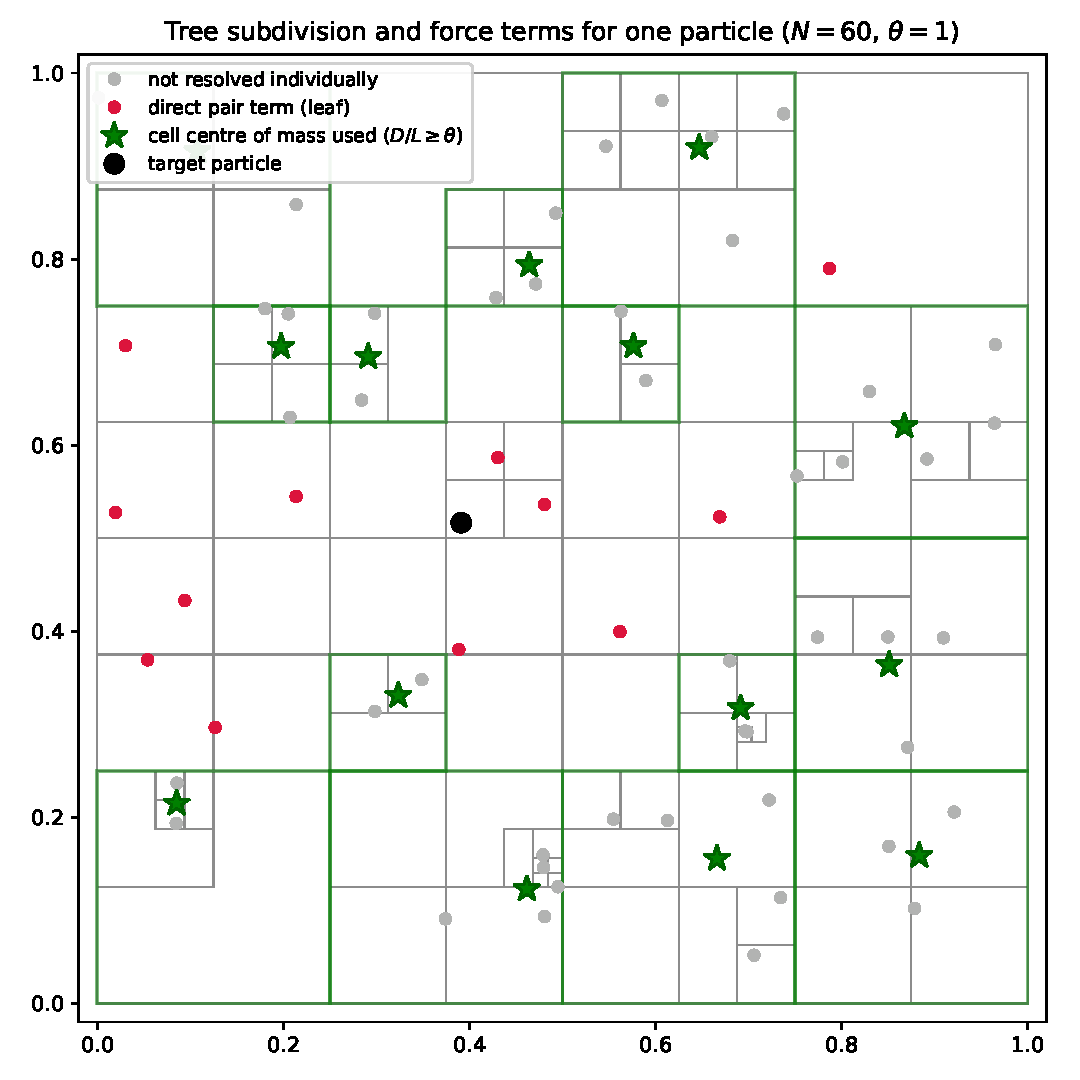
\includegraphics[width=0.72\textwidth]{figures/fig_tree.pdf}
 \caption{Two-dimensional illustration of the tree method with $\theta=1$.
 Thin lines are cell boundaries. Red points contribute a direct pair force to
 the black target particle. Green stars are cell centers of mass that satisfy
 $D/L\geq\theta$, drawn inside the cell they replace. Grey points are absorbed
 into those cells.}
 \label{fig:tree}
\end{figure}

\subsection{Adaptive RK4 integration}

The solver represents the state as
$\mathbf{y}=(\mathbf{r}_1,\ldots,\mathbf{r}_N,
\mathbf{v}_1,\ldots,\mathbf{v}_N)$ and integrates
\begin{equation}
 \dot{\mathbf{r}}_i=\mathbf{v}_i,
 \qquad \dot{\mathbf{v}}_i=\mathbf{a}_i.
\end{equation}
For a proposed interval $h$, the controller compares one fourth-order
Runge-Kutta step with two steps of length $h/2$. Their identical first stage is
reused, so the comparison costs eleven force evaluations. The brief defines the
error as the largest particle
displacement difference,
\begin{equation}\label{eq:errnorm}
 \mathrm{err}=\max_i\norm{\mathbf{r}_{i,\mathrm{half}}
 -\mathbf{r}_{i,\mathrm{full}}}.
\end{equation}
The controller accepts the step when $\mathrm{err}\leq\mathrm{tol}$ and applies
Richardson extrapolation,
\begin{equation}
 \mathbf{y}_{\mathrm{acc}}=\mathbf{y}_{\mathrm{half}}+
 \frac{\mathbf{y}_{\mathrm{half}}-\mathbf{y}_{\mathrm{full}}}{2^4-1}.
\end{equation}
The controller multiplies $h$ by
$0.9(\mathrm{tol}/\mathrm{err})^{1/5}$, with a maximum growth factor of
two and a minimum reduction factor of $0.1$. Error control keeps the proposed
step between $0.01$ and $\SI{2}{Gyr}$. Clipping at a reporting time can reduce
an accepted interval below this limit. The following one or two intervals may
also remain short because $h$ grows by at most a factor of two per accepted
step. The shortest interval in the production runs is \SI{0.0016}{Gyr}. If the
error still exceeds the tolerance at the lower bound, the solver stops rather
than accept an uncontrolled step.

The brief sets the displacement accuracy to $\varepsilon=0.1$ in units of the
box size, yielding
\begin{equation}\label{eq:tolliteral}
 \mathrm{tol}=\varepsilon L_{\mathrm{box}}=0.1\times\SI{1332}{kpc}
 =\SI{133.2}{kpc},
\end{equation}
a permitted step error of \SI{133}{kpc} for an initial cluster radius of
\SI{50}{kpc}. Section~\ref{sec:tolerance} tests this value.

The integration begins at 0 Gyr and clips steps to land exactly at 2.5, 5, 10,
15, and \SI{20}{Gyr}, so each stored snapshot matches its label.

\subsection{Energy and escapers}

At every accepted step, the energy diagnostic calculates
\begin{equation}\label{eq:energy}
 E_k=\frac12\sum_i m_i v_i^2,
 \qquad E_g=\frac12\sum_i m_i\Phi_i,
 \qquad \Phi_i=-G\sum_{j\ne i}\frac{m_j}{r_{ij}+S}.
\end{equation}
For $N>1500$, the diagnostic evaluates $\Phi_i$ with the force tree; smaller
tests use the direct sum. When particles leave, the code stores their kinetic
energy and estimates $E_g$ before and after removal. Their difference includes
escaper-escaper and escaper-retained terms within the chosen estimator. At
production size, both estimates use separate Barnes-Hut approximations. The
retained curve includes only active particles; the corrected curve adds the
frozen escape contributions. Neither includes later interactions because
removed particles no longer evolve. The removal rule is geometric, so escaper
here means boundary-removed rather than proven unbound: at $V=80$, 21 of the
123 removal events left with non-positive $E_k+E_g$.

\subsection{Density profile and King fit}

Radii are measured from the retained center of mass, which is displaced by 2 to
8 kpc after escaper removal. The occupied radial range is divided into 25
logarithmic shells.
For shell edges $r_j$ and $r_{j+1}$,
\begin{equation}
 \rho_j=\frac{M_j}{\frac{4\pi}{3}(r_{j+1}^3-r_j^3)},
 \qquad r_{j,\mathrm{plot}}=\sqrt{r_jr_{j+1}}.
\end{equation}
For equal mass particles, the Poisson uncertainty is
$\delta\rho_j=\rho_j/\sqrt{N_j}$. The implementation also supports unequal
masses by summing $m_i^2$ in each shell.

The fit uses the model requested in the assignment,
\begin{equation}\label{eq:king}
 \rho(r)=\frac{\rho_c}{[1+(r/r_c)^\alpha]^\beta}.
\end{equation}
The analysis fits $\log\rho$ with propagated error
$\delta\log\rho\simeq\delta\rho/\rho$. Optimizing $\log\rho_c$ and
$\log r_c$ keeps both parameters positive. The $V=80$ fit scans several
starting values for $\alpha$ and $\beta$, then holds them fixed while fitting
$\rho_c$ and $r_c$ for $V=65$ and $V=95$.

\section{Implementation and checks}\label{sec:implementation}

The submitted \texttt{nbody\_solver.py} implements sampling, tree forces,
adaptive integration, diagnostics, fitting, plotting, and self-tests. Numba
compiles the flattened tree and distributes target particles across threads;
the Python walk is the fallback. The RK controller from HW\_05 uses the
per-particle norm in Equation~\ref{eq:errnorm} and resizes the state after
escapes. The isotropic direction sampler comes from HW\_07.

The command \texttt{python nbody\_solver.py -{}-test} runs the checks, and
\texttt{-{}-tol=X} runs all three $N=5000$ cases. Outputs are stored under
\texttt{figures/}; redraw and refit modes reuse saved states without repeating
the dynamics.

In the self-test, 5000 samples give a maximum radius of \SI{49.9905}{kpc} and
an RMS speed of \SI{79.422}{km/s} for the \SI{80}{km/s} distribution. The
production draw gives \SI{49.9961}{kpc} and \SI{80.235}{km/s}. These
sub-percent deviations match sampling noise, and subtracting the mean sets the
center-of-mass velocity to machine zero.

For 150 particles with unequal masses, the Barnes-Hut acceleration at
$\theta=1$ had a relative error
$\norm{\mathbf{a}_{\mathrm{tree}}-\mathbf{a}_{\mathrm{dir}}}/
\norm{\mathbf{a}_{\mathrm{dir}}}=1.014\times10^{-2}$ against the direct sum,
with both norms stacked over all particles and components. The tree
gravitational energy differed from the direct result by
$5.214\times10^{-4}$. A softened unequal-mass circular binary completed two
periods with a relative energy change of $1.29\times10^{-10}$ under a tight
tolerance, and its final separation agreed with the initial value to the
reported precision. A separate constant-velocity test confirmed that stored
snapshots match their labels.

The brief's opening convention differs from the standard side-length form.
Since $L=\sqrt3\,l$,
\begin{equation}\label{eq:thetaconv}
 \frac{D}{L}\geq\theta_{\mathrm{diagonal}}
 \quad\Longleftrightarrow\quad
 \frac{l}{D}\leq
 \frac{1}{\sqrt3\,\theta_{\mathrm{diagonal}}}
 \equiv\theta_{\mathrm{side}}.
\end{equation}
Table~\ref{tab:theta} compares the tree acceleration with a direct sum for
3000 particles. At the assigned $\theta=1$, the $L_2$ error is
$9.14\times10^{-3}$, consistent with the smaller random test.

\begin{table}[htbp]
 \centering
 \caption{Barnes-Hut acceleration error against direct summation for the
 initial uniform sphere, $N=3000$.}
 \label{tab:theta}
 \input{figures/theta_table.tex}
\end{table}

Raising $\theta$ to 2 cuts the error by a factor of eight. At $N=5000$, tree
construction dominates the runtime, so changing $\theta$ has little effect. The
production runs use the assigned $\theta=1$.

The production controller accepted 310, 262 and 352 steps for $V=80$, $95$
and \SI{65}{km/s}, with 4, 10 and 3 rejected proposals. The assigned tolerance
produced no rejections in the corresponding full runs.

\section{Choice of integration tolerance}\label{sec:tolerance}

The assigned tolerance, \SI{133.2}{kpc}, exceeds the initial cluster radius.
The tolerance study repeats the $V=\SI{80}{km/s}$ run at four values across
three decades. For each run, the energy diagnostic measures the retained
particle energy plus the escape values frozen at removal. Adding these values
removes deletion jumps but does not make the diagnostic exact: the Barnes-Hut
force and tree energy both introduce spatial approximations. Comparing the runs
measures sensitivity to timestep error while these approximations remain at
every tolerance.

\begin{table}[htbp]
 \centering
 \caption{Energy drift versus RK4 position tolerance for $V=\SI{80}{km/s}$,
 $N=5000$, \SI{20}{Gyr}, including frozen escape values.}
 \label{tab:tolerance}
 \input{figures/conv_table.tex}
\end{table}

\begin{figure}[htbp]
 \centering
 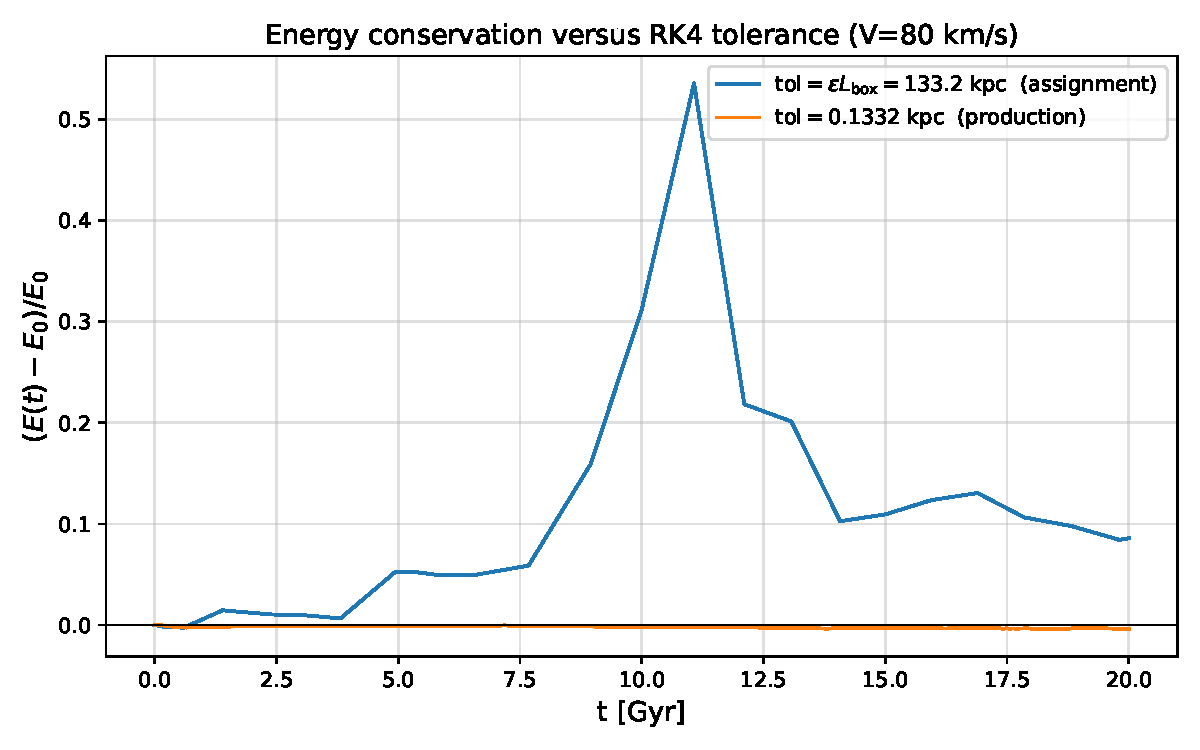
\includegraphics[width=0.86\textwidth]{figures/fig_tolerance.pdf}
 \caption{Relative energy change for $V=\SI{80}{km/s}$ at the tolerance of the
 assignment and at the tolerance used for the production runs.}
 \label{fig:tolerance}
\end{figure}

Tightening the tolerance to \SI{0.1332}{kpc} lowers the worst energy excursion
from 48 percent to 0.25 percent while increasing the step count from 20 to 303.
The main results use this value; Appendix~\ref{sec:appendixeps} provides every
required output at the assigned tolerance under the suffix \texttt{\_eps01}.

The drift falls at every row of Table~\ref{tab:tolerance}, so the study does not
reach a floor. Further tightening would eventually expose
timestep-independent tree and close-encounter errors, but these runs do not
locate that crossover.

\section{Results}\label{sec:results}

\subsection{Initial energies}

For an unsoftened uniform sphere,
$E_g=-3GM^2/(5R)$. Since $E_k=MV^2/2$, the virial value $2E_k/\abs{E_g}=1$
occurs at
\begin{equation}
 V_{\mathrm{vir}}=\sqrt{\frac{3GM}{5R}}=\SI{71.85}{km/s}.
\end{equation}
The $V=65$ case starts below virial equilibrium, while the $V=80$ and
$V=95$ cases start above it. All three have $2E_k/\abs{E_g}<2$ and negative
initial total energy. The $V=95$ state is close to zero energy, but it is not
initially unbound.

\begin{table}[htbp]
 \centering
 \caption{Initial and final run data. Energies use the simulation units.}
 \label{tab:runs}
 \begin{tabular}{cccccc}
 \toprule
 $V$ [km/s] & $2E_{k,0}/\abs{E_{g,0}}$ &
 $E_0$ [$10^{14}M_\odot\,\mathrm{kpc}^2\,\mathrm{Gyr}^{-2}$] &
 removed & retained & steps \\
 \midrule
 65 & 0.849 & $-3.013$ & 20 & 4980 & 352 \\
 80 & 1.286 & $-1.868$ & 167 & 4833 & 310 \\
 95 & 1.814 & $-0.488$ & 758 & 4242 & 262 \\
 \bottomrule
 \end{tabular}
\end{table}

\subsection{(a) Particle positions}

Figure~\ref{fig:positions} shows the $V=80$ positions at the six requested
times. The panels frame the cluster because the full box would hide its
structure. By \SI{2.5}{Gyr}, the uniform sphere has formed a dense core and an
extended halo. The halo expands throughout the run, and 167 particles cross
the box boundary.

\begin{figure}[p]
 \centering
 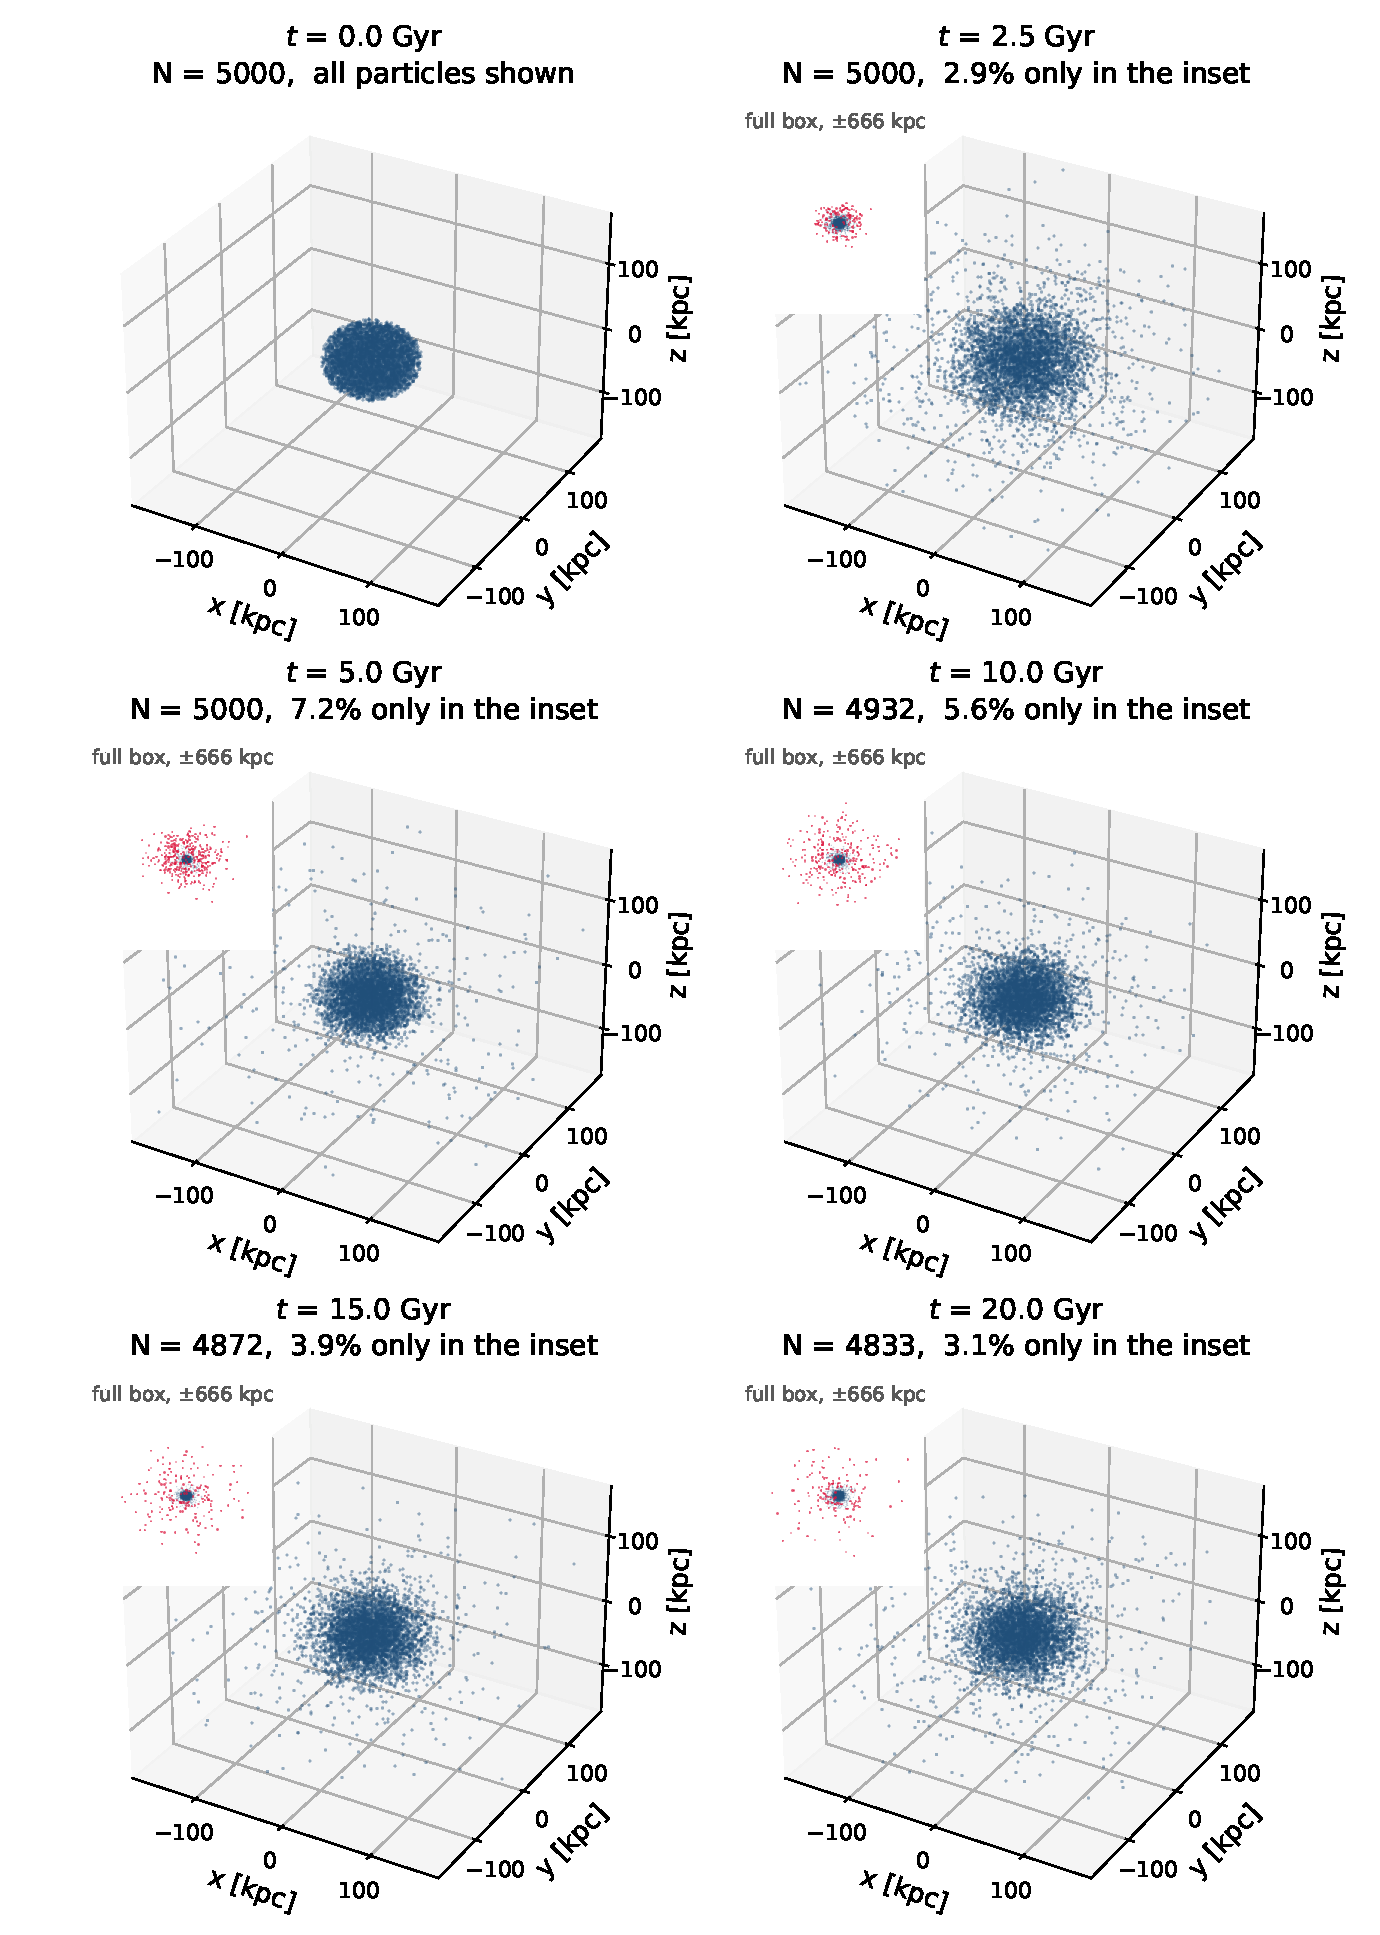
\includegraphics[width=\textwidth]{figures/fig_a.pdf}
 \caption{Particle positions for the $V=\SI{80}{km/s}$ run. Each panel shows
 an integrated state at the time printed above it.}
 \label{fig:positions}
\end{figure}

\subsection{(b) Energy conservation}

The curves in Figure~\ref{fig:energy} separate after the first escape at
\SI{5.3}{Gyr}. Since $E_0<0$, a positive value of $(E-E_0)/E_0$ means the total
energy has become more negative. At \SI{20}{Gyr}, the retained energy gives
$+0.034$ and the frozen-escape accounting gives $-0.0039$. The removed
particles carry away kinetic energy equal to 4.6 percent of $\abs{E_0}$, but
only 0.8 percent in negative interaction energy. The retained total therefore
becomes more negative and its relative-change curve rises. At $V=95$, where
758 particles escape, the two final values
are $+0.81$ and $+0.0013$; the corrected curve peaks at $0.0069$ earlier in the
run. At $V=65$, only 20 leave; the retained and corrected values end at
$-0.0020$ and $-0.0032$.

\begin{figure}[htbp]
 \centering
 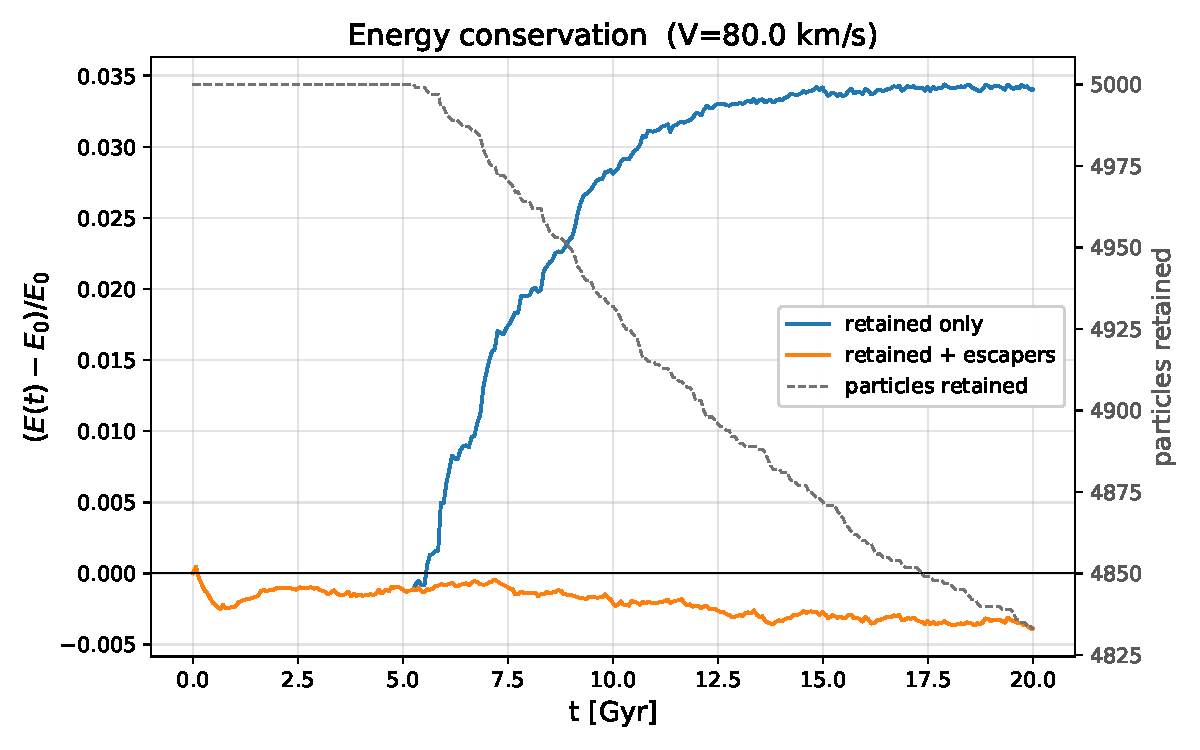
\includegraphics[width=0.86\textwidth]{figures/fig_b.pdf}
 \caption{Relative energy change for $V=\SI{80}{km/s}$. Blue uses retained
 particles, orange restores each escaper's energy recorded at removal, and the
 dashed grey line gives the retained count on the right axis.}
 \label{fig:energy}
\end{figure}

\subsection{(c) Virial ratio}

The $V=80$ ratio starts at $1.286$, falls to $0.82$ by \SI{2.5}{Gyr}, and then
oscillates about one with decreasing amplitude (Figure~\ref{fig:virial}).
Maxima at 5.1, 9.4, 14.0 and \SI{18.6}{Gyr} give a \SI{4.5}{Gyr} period. The
final retained value is $0.954$. The damped oscillation toward unity is
consistent with violent relaxation.

The final retained ratios are $0.960$, $0.954$ and $0.937$ for $V=65$, $80$ and
$\SI{95}{km/s}$. The $V=65$ system starts at $0.849$, contracts, and loses 20
particles. The $V=95$ system starts at $1.814$ and loses 15 percent of its mass
as it approaches equilibrium. Its two escape-accounting curves differ most.

The plotted ratio $-2E_k/E_g$ is the virial condition requested in the brief,
which holds exactly for an unsoftened potential. Since
$U_{ij}\propto(r_{ij}+S)^{-1}$ is not homogeneous of degree $-1$, the
softening-consistent statement is $2E_k+W=0$ with
$W=\sum_{i<j}\mathbf{r}_{ij}\cdot\mathbf{f}_{ij}
=-\sum_{i<j}Gm_im_jr_{ij}/(r_{ij}+S)^2$. Summing $W$ directly over the final
states gives $2E_k/\abs{W}=0.9996$, $0.982$ and $0.956$ for $V=65$, $80$ and
\SI{95}{km/s}, closer to unity than the plotted values in all three runs.

\begin{figure}[htbp]
 \centering
 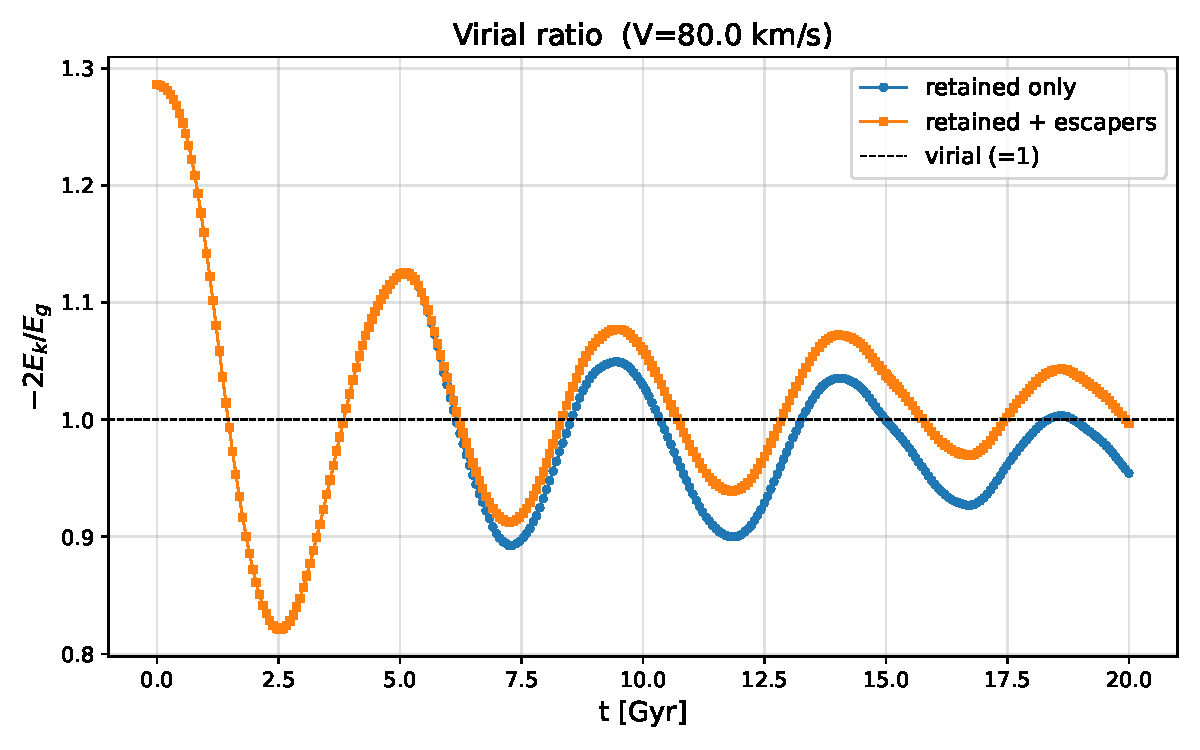
\includegraphics[width=0.86\textwidth]{figures/fig_c.pdf}
 \caption{Virial ratio for $V=\SI{80}{km/s}$. The horizontal line marks
 $-2E_k/E_g=1$.}
 \label{fig:virial}
\end{figure}

\subsection{(d) Density profiles and King fits}

The fitted core radius increases monotonically with initial velocity, from
\SI{24.7}{kpc} at $V=65$ through \SI{35.1}{kpc} at $V=80$ to \SI{57.4}{kpc}
at $V=95$. The central density falls by more than a factor of ten over the same
range, from $7.5\times10^5$ to $5.4\times10^4\,M_\odot\,\mathrm{kpc}^{-3}$.
Higher initial velocity leaves a larger, more diffuse remnant
(Figure~\ref{fig:density}).

\begin{figure}[htbp]
 \centering
 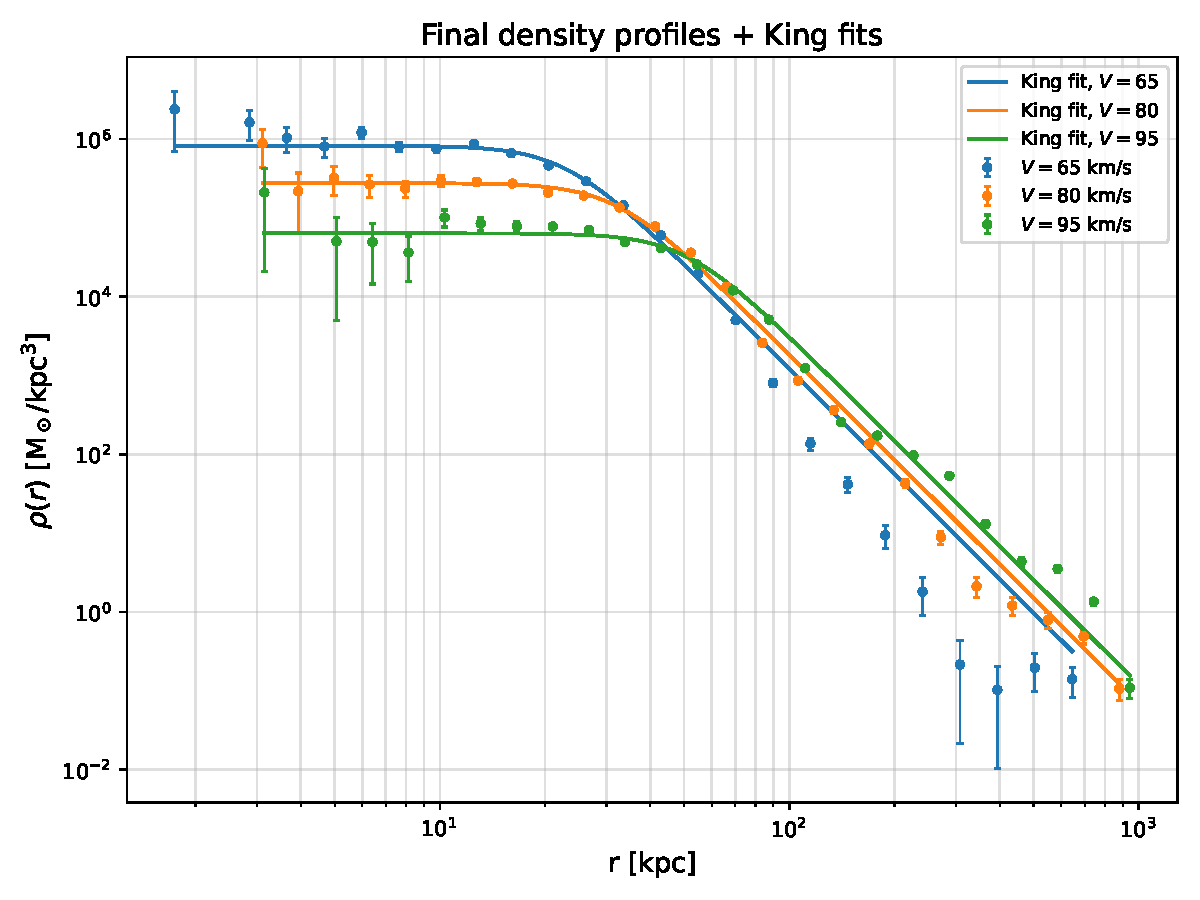
\includegraphics[width=0.82\textwidth]{figures/fig_d.pdf}
 \caption{Center-of-mass density profiles at \SI{20}{Gyr} with King-model
 fits. The $V=65$ and $V=95$ fits use the $\alpha$ and $\beta$ values obtained
 from $V=80$.}
 \label{fig:density}
\end{figure}

\begin{table}[htbp]
 \centering
 \caption{King-model parameters. The uncertainties are the formal
 one-standard-deviation errors from the weighted fit. For $V=65$ and $95$ they
 are conditional on the $\alpha$ and $\beta$ held fixed from $V=80$.}
 \label{tab:king}
 \input{figures/king_table.tex}
\end{table}

The common shape parameters are $\alpha=4.83\pm0.38$ and
$\beta=0.986\pm0.085$. The outer profile constrains their product because
$\rho\propto r^{-\alpha\beta}$ at large radius. Here $\alpha\beta=4.77$, close
to the Plummer value of 5. The assigned-tolerance states give
$\alpha=0.700$, $\beta=7.389$, and a similar product of $5.17$. The data
therefore constrain the outer slope more strongly than either shape parameter.

The reduced $\chi^2$ values, $7.7$, $44.7$ and $12.8$ for $V=80$, $95$ and
\SI{65}{km/s}, exceed unity. Populated bins have small Poisson errors, so
departures from the King form dominate the statistic; the $V=95$ profile also
has a shallow central depression that a monotonic King curve cannot fit. The
quoted uncertainties describe local parameter curvature, not model mismatch.

\FloatBarrier
\section{Numerical difficulties}\label{sec:difficulties}

The assigned tolerance exceeds the initial cluster diameter and permits energy
errors of tens of percent (Section~\ref{sec:tolerance}). RK4 is non-symplectic and
therefore lacks the bounded long-time energy error typical of leapfrog methods.
The drift decreases at every tested tolerance. The Barnes-Hut force and energy
approximations do not depend on the timestep, and these runs do not locate the
tree- and encounter-dominated error floor.

Close encounters raise the acceleration and can drive the step to its
\SI{0.01}{Gyr} floor. Softening bounds the pair force by $Gm_im_j/S^2$; if the
error remains too large at the floor, the code stops rather than accepting an
uncontrolled step. Exact coordinate duplicates require a separate tree-build
guard because repeated octant subdivision cannot separate them. The tree stores
such particles in one childless cell. The group acts as a single point mass for
an external target, which is exact. Their mutual force is set to zero, which is
a regularization rather than an evaluation of Equation~\ref{eq:softforce}: at
$r_{ij}=0$ that law has finite magnitude $Gm_im_j/S^2$ and undefined direction.
The chosen initial sampler does not generate duplicates.

Computing $E_g$ with the $\theta=1$ tree walk costs $O(N\log N)$ at every
accepted step. Its relative bias is $5.2\times10^{-4}$ against the direct sum
for 150 particles, below the measured drift; runs below 1500 particles use the
exact sum. Escaper removal causes jumps in the retained-particle energy by
deleting both the particle's kinetic energy and its pair terms. The corrected
curves in Figures~\ref{fig:energy} and~\ref{fig:virial} remove these jumps from
the plotted diagnostics, but retain tree-estimator error and omit post-removal
interactions.

For the density fit, 25 logarithmic shells resolve the core better than a linear
grid; empty bins are omitted and the remaining points use Poisson weights.
Because the outer model mainly constrains $\alpha\beta$, the log-space fit tries
several starting points and retains the lowest $\chi^2$. Fixing the $V=80$ shape
for the other two velocities reduces this degeneracy and satisfies the
assignment.

Adaptive step doubling needs eleven force evaluations per attempted step
because the full step and first half step reuse their identical first stage.
Each remaining force evaluation builds a new tree. Flattened tree arrays, a
Numba-compiled walk and
threaded target-particle loops make the $N=5000$ calculation tractable.

\FloatBarrier
\section{Conclusion}\label{sec:conclusion}

Direct-sum tests validate the tree calculation; softened-binary and snapshot
tests validate the integrator. After \SI{20}{Gyr}, all three systems approach
$-2E_k/E_g\approx1$: the \SI{65}{km/s} system contracts and
retains almost all its mass, while the \SI{80}{km/s} and \SI{95}{km/s} systems
expand and lose about 3 and 15 percent. Their fitted core radii increase and
central densities decrease with initial speed.

At the assigned \SI{133.2}{kpc} tolerance, final escape-corrected energy shifts
range from 9 to 35 percent.
Reducing it by $10^3$ brings all three final shifts below 0.4 percent, and the
largest excursion at any time below 0.7 percent, at the cost of 310 rather than
28 accepted steps for the full-output \SI{80}{km/s} case. The main results
therefore use the tighter tolerance; Appendix~\ref{sec:appendixeps} retains
every requested output at the assigned value.

\appendix
\section{Results at the assigned tolerance}\label{sec:appendixeps}

This appendix repeats all three runs with the assigned
$\mathrm{tol}=\varepsilon L_{\mathrm{box}}=\SI{133.2}{kpc}$ instead of the
tighter \SI{0.1332}{kpc}. The files use the \texttt{\_eps01} suffix and the
command
\begin{center}
 \texttt{python nbody\_solver.py -{}-tol=133.2 -{}-tag=eps01}.
\end{center}
The initial conditions, $\theta$, $S$, box, and end time are unchanged.

The controller accepts 28, 15 and 34 steps for $V=80$, $95$ and
\SI{65}{km/s}, with no rejections. The tolerance study in
Table~\ref{tab:tolerance} uses a smaller step floor and no intermediate snapshot
times, so its accepted sequence and drift differ slightly. In both
configurations, the tolerance exceeds the initial cluster diameter and provides
little step control.

\begin{table}[htbp]
 \centering
 \caption{Assigned and tighter runs. $\Delta E/E_0$ is the final value of the
 escaper-corrected relative energy change, not its largest excursion; the
 assigned-tolerance $V=80$ run peaks at $0.54$ and the tighter $V=95$ run at
 $0.007$.}
 \label{tab:epscompare}
 \begin{tabular}{lcccccc}
 \toprule
 & \multicolumn{3}{c}{$\mathrm{tol}=\SI{133.2}{kpc}$ (assigned)}
 & \multicolumn{3}{c}{$\mathrm{tol}=\SI{0.1332}{kpc}$ (used)} \\
 \cmidrule(lr){2-4}\cmidrule(lr){5-7}
 $V$ [km/s] & steps & retained & $\Delta E/E_0$ &
 steps & retained & $\Delta E/E_0$ \\
 \midrule
 65 & 34 & 4755 & $-0.347$ & 352 & 4980 & $-0.003$ \\
 80 & 28 & 4822 & $+0.086$ & 310 & 4833 & $-0.004$ \\
 95 & 15 & 4239 & $+0.219$ & 262 & 4242 & $+0.001$ \\
 \bottomrule
 \end{tabular}
\end{table}

\begin{figure}[p]
 \centering
 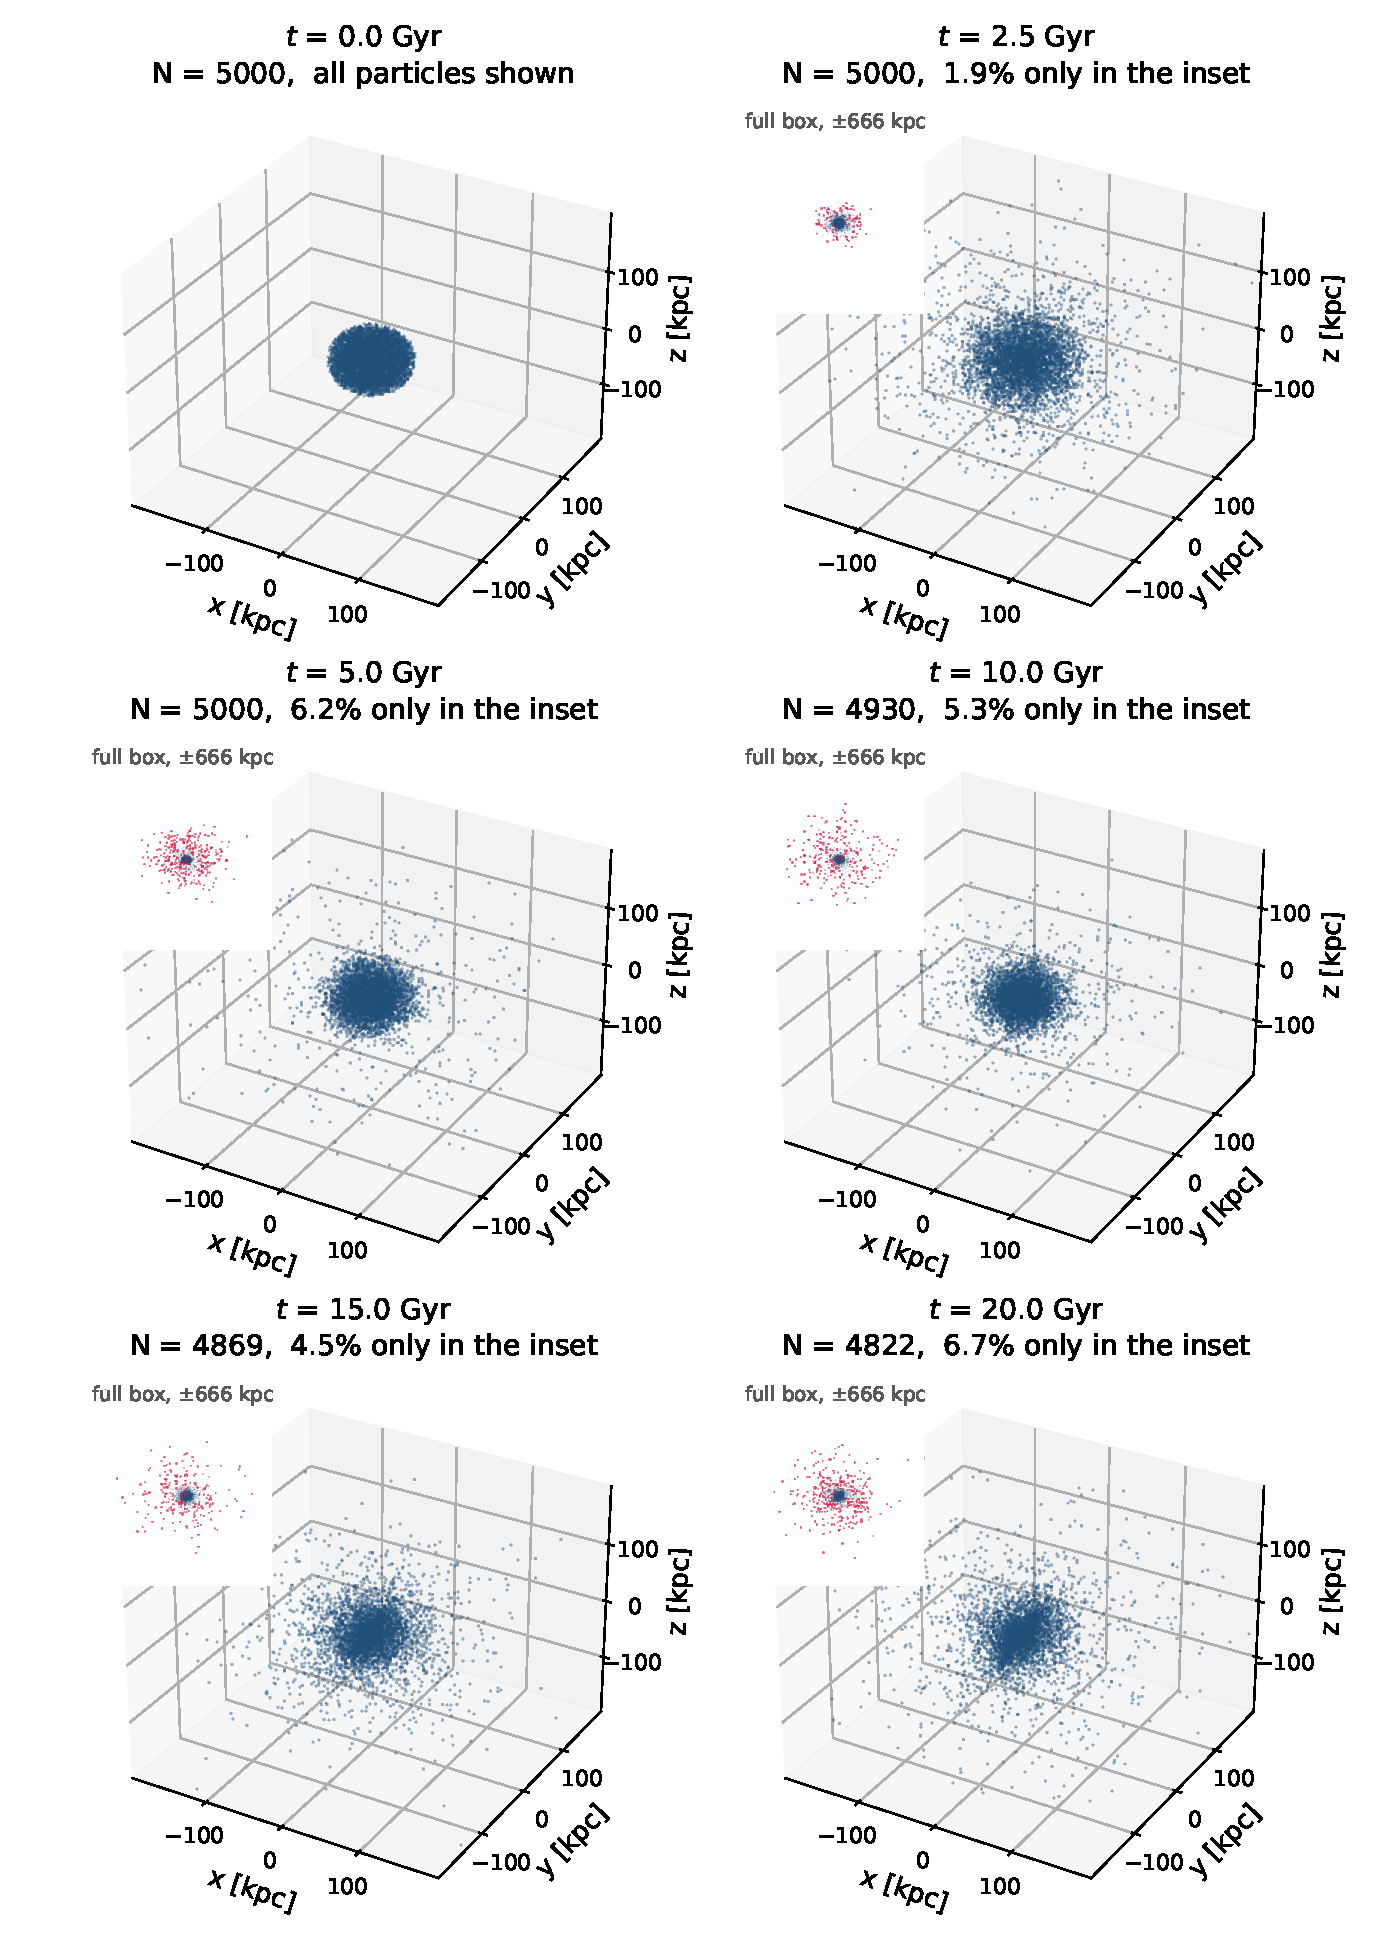
\includegraphics[width=\textwidth]{figures/fig_a_eps01.pdf}
 \caption{Assigned-tolerance particle positions for $V=\SI{80}{km/s}$,
 requirement (a).}
 \label{fig:positions_eps}
\end{figure}

\begin{figure}[htbp]
 \centering
 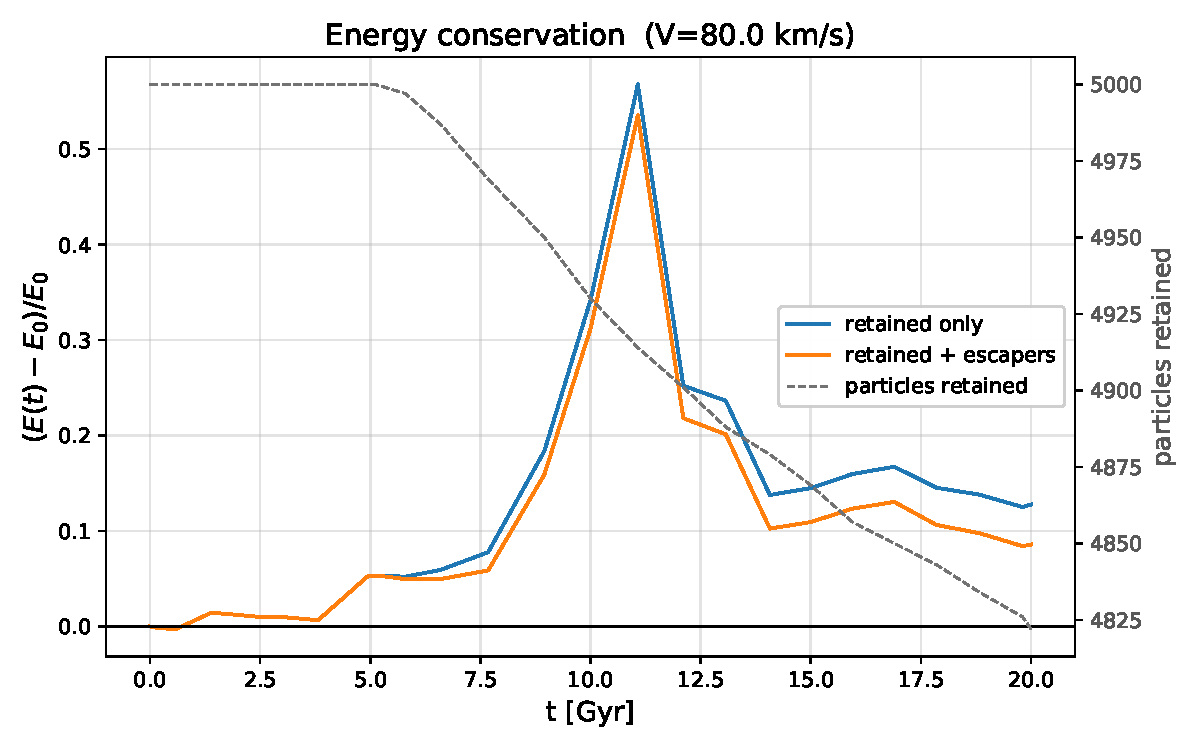
\includegraphics[width=0.86\textwidth]{figures/fig_b_eps01.pdf}
 \caption{Assigned-tolerance energy and population for $V=\SI{80}{km/s}$,
 requirement (b).}
 \label{fig:energy_eps}
\end{figure}

\begin{figure}[htbp]
 \centering
 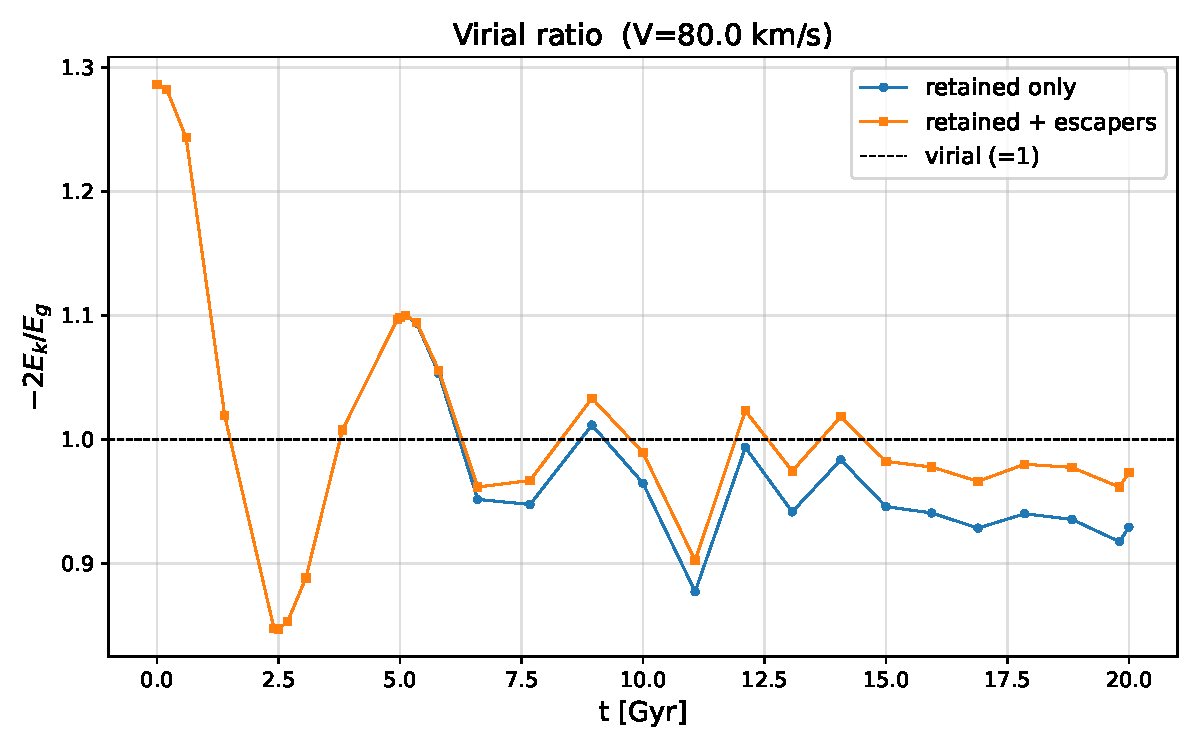
\includegraphics[width=0.86\textwidth]{figures/fig_c_eps01.pdf}
 \caption{Assigned-tolerance virial ratio for $V=\SI{80}{km/s}$,
 requirement (c).}
 \label{fig:virial_eps}
\end{figure}

\begin{figure}[htbp]
 \centering
 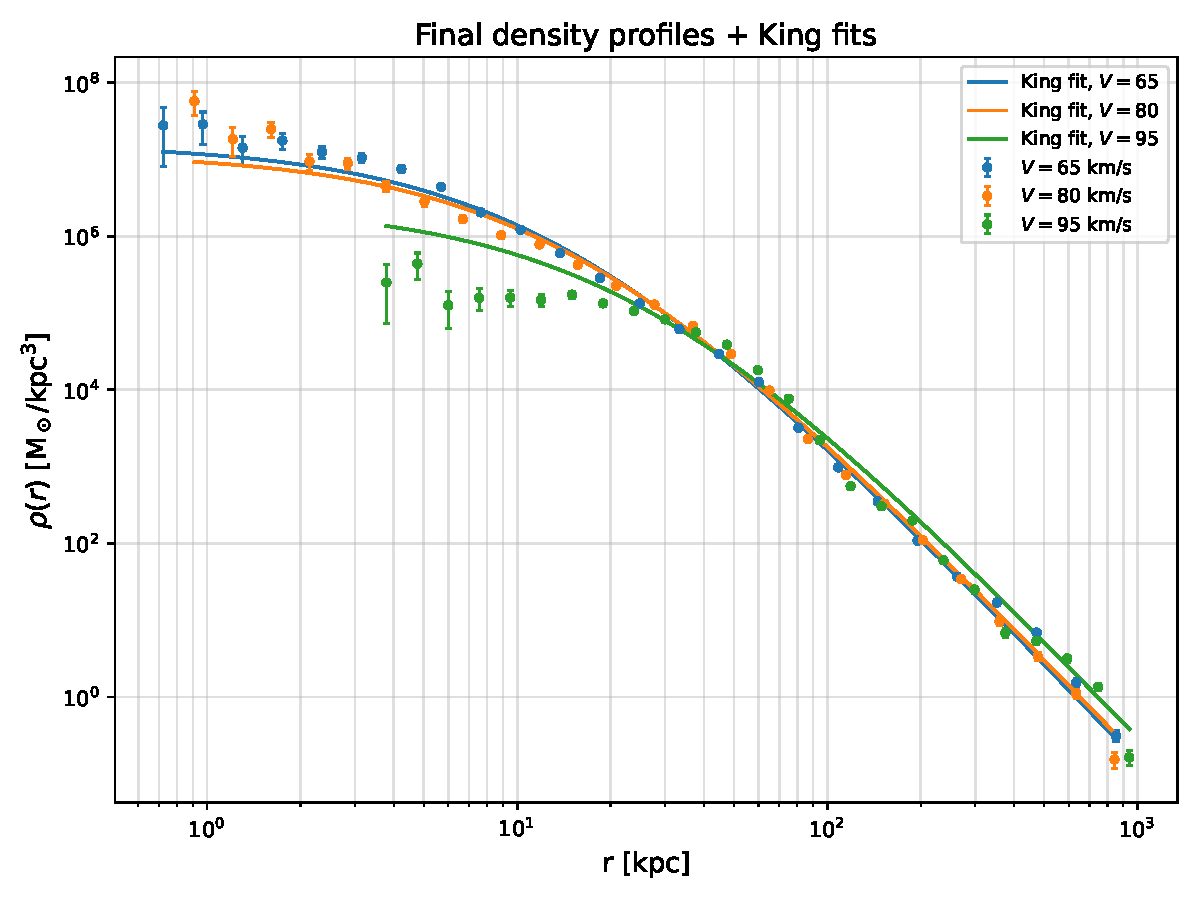
\includegraphics[width=0.82\textwidth]{figures/fig_d_eps01.pdf}
 \caption{Assigned-tolerance density profiles and King fits, requirement (d).}
 \label{fig:density_eps}
\end{figure}

\begin{table}[htbp]
 \centering
 \caption{Assigned-tolerance King parameters. The $V=80$ fit supplies
 $\alpha$ and $\beta$ for the other velocities.}
 \label{tab:king_eps}
 \input{figures/king_table_eps01.tex}
\end{table}

At the assigned tolerance, the corrected energy error reaches 54 percent in the
full-output $V=80$ run. Table~\ref{tab:tolerance} gives 48 percent because a
different step floor and output schedule alter the accepted sequence. The
virial ratio ends near unity, $0.929$ rather than $0.954$, but its 28 samples
cannot resolve the \SI{4.5}{Gyr} period.

The density fits are less reliable. Table~\ref{tab:king_eps} gives
$r_c=24.5$, $25.2$ and \SI{40.0}{kpc} for $V=65$, $80$ and \SI{95}{km/s}; the
first two agree within error, erasing the tighter-run trend. At
\SI{65}{km/s}, the coarse cusp raises the central density from $\num{7.5e5}$ to
$\num{2.9e7}\,M_\odot\,\mathrm{kpc}^{-3}$. Although $(\alpha,\beta)$ changes
from $(4.831,0.986)$ to $(0.700,7.389)$, their product remains close, 4.77 versus
5.17. The loose run removes 245 particles instead of 20.

\FloatBarrier
\addcontentsline{toc}{section}{References}
\begin{thebibliography}{9}
\bibitem{barneshut} J. Barnes and P. Hut, ``A hierarchical $O(N\log N)$
force-calculation algorithm,'' \textit{Nature} \textbf{324}, 446--449 (1986).
\end{thebibliography}

\end{document}
